
\section{Example: Cantilevered Beam}
Another physical system that has a response that can be approximated by our second-order model is a cantilevered beam.  Imagine a yardstick fixed on one end.  When the free end is subject to a displacement (the initial condition) and then released, the tip will oscillate.  A cantilevered beam, unlike our lumped mass system in Figure~\ref{f:msd2}, is a continuous system, but for now we'll approximate it by examining the first natural frequency.  

\subsection{First-Mode of Cantilevered Beam}
The first natural frequency of a uniform cantilevered beam, Figure~\ref{f:blevins}, can be estimated by using classical beam theory.
\begin{figure}[htb!]
\centerline{
{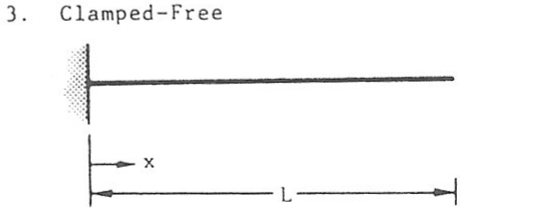
\includegraphics[width=0.4\textwidth]{blevins_beam.png}}}
\caption{Image of a cantilevered beam model.  From ``Formulas for Natural Frequency and Mode Shape'' by R. D. Blevins.}
\label{f:blevins}
\end{figure}
The resulting expression for the first natural frequency, in \unitfrac[]{rad}{s}, is
\begin{equation}\label{e:blevins}
\omega_n = \frac{(1.875)^2}{L^2} \sqrt{\left( \frac{EI}{\rho} \right)}
\end{equation}
where $\rho$ is the mass per unit length of the beam (the product of the density and the cross-section area), $E$ is the modulus of elasticity of the beam material, $I$ is the second moment of area of the beam and $L$ is the length of the beam. 

\subsection{First-Mode of Cantilevered Beam with Added Mass}
Similarly, it is possible to predict the natural frequency of a uniform cantilevered beam with a point-mass at the free end of the beam as illustrated in Figure~\ref{f:blevinsmass}.
\begin{figure}[htb!]
\centerline{
{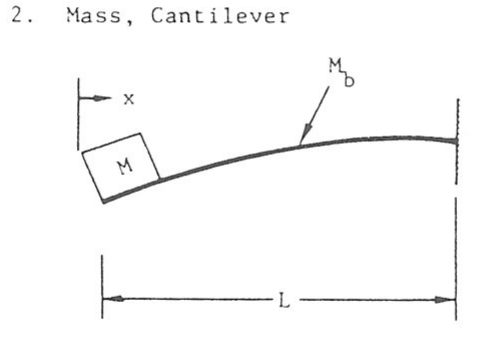
\includegraphics[width=0.4\textwidth]{blevins_beam_mass.png}}}
\caption{Image of a cantilevered beam with point mass model from ``Formulas for Natural Frequency and Mode Shape'' by R. D. Blevins.}
\label{f:blevinsmass}
\end{figure}
The first natural frequency for this model is
\begin{equation}\label{e:blevinsmass}
\omega_n = \sqrt{ \frac{3 E I}{L^3 (M+0.24 M_b)}}
\end{equation}
where $M$ is the point mass at the free end of the beam and $M_b$ is the total mass of the beam.

Notice that both predicted natural frequencies (\ref{e:blevins}) and (\ref{e:blevinsmass}) have the general from of $\omega_n = \sqrt{K/M}$ where $K$ is the ``stiffness'' of the system and $M$ is the ``mass'' of the system.


\begin{ex}\label{ex:beamvib}
Given a uniform cantilevered beam with the following properties:
\begin{itemize}
\item Length = \unit[0.5]{m}
\item Width = \unit[2.54]{cm}
\item Thickness = \unit[1.59]{mm}
\item Modulus of Elasticity ($E$) = \unit[68.9]{GPa}
\item Density = \unitfrac[2.70]{g}{cm$^3$}
\end{itemize}
Predict the undamped natural frequency.  Express the answer in both of the following units: \unitfrac[]{rad}{s} and \unit[]{Hz}.
\end{ex}

\ifsolutions
\begin{soln}
Use (\ref{e:blevins}) with the values from the Exercise.  The mass-per-unit-length is the product of the density and the cross-sectional area:
\[ \rho = D*(t*W) \]
where $D$ is the density, $t$ is the beam thickness and $W$ is the beam width.
We also need to calculate the second moment of area...
\[ I = 1/12(W*t^3) \]
If we plug in these values we get...
\[ \omega_n = \unitfrac[32.6]{rad}{s} \]
To express in Hz
\[ f_n = \frac{\unitfrac[\omega_n]{rad}{s}}{\unitfrac[2\pi]{rad}{cycle}} = \unitfrac[5.2]{cycles}{s}=\unit[5.2]{Hz}
\]

\lstinputlisting[style=myMatStyle,
caption={Script for predicting the natural frequency of a cantilevered beam.},
label={l:natlfreq}]
{../code/natl_freq_pred.m}

\end{soln}
\fi

\begin{ex}\label{ex:model2sim}
Given the uniform cantilevered beam described in the previous example, and a damping ratio of $\zeta=0.02$ (2\% damping)...
\begin{itemize}
\item Write an expression for a mathematical model of the form in (\ref{e:second}) to describe the system.  (You should just need to substitute in numerical values for the system parameters $\zeta$ and $\omega_n$.)
\item Using MATLAB, produce a graph that predicts the response of the tip of the cantilevered beam to an initial displacement of \unit[1.0]{cm} and zero initial velocity: $y(0)=\unit[1.0]{cm}$ and $\dot{y}(0) = \unitfrac[0]{cm}{s}$.
\end{itemize}
\end{ex}

\ifsolutions
\begin{soln}
\[
\ddot{y}(t) + 2 (0.02) (32.6)\dot{y}(t) + (32.6)^2 = f(t)
\]
To generate the graph we can use the same script from Exercise~\ref{ex:secondresp} and substitute in the new values for $\zeta$ and $\omega_n$.

\lstinputlisting[style=myMatStyle,
caption={Script for plotting the corrected free response of a second-order model using the given beam parameters.},
label={l:secondfreemodelsoln}]
{../code/second_order_free_model.m}

\begin{figure}[hbt]
\centering
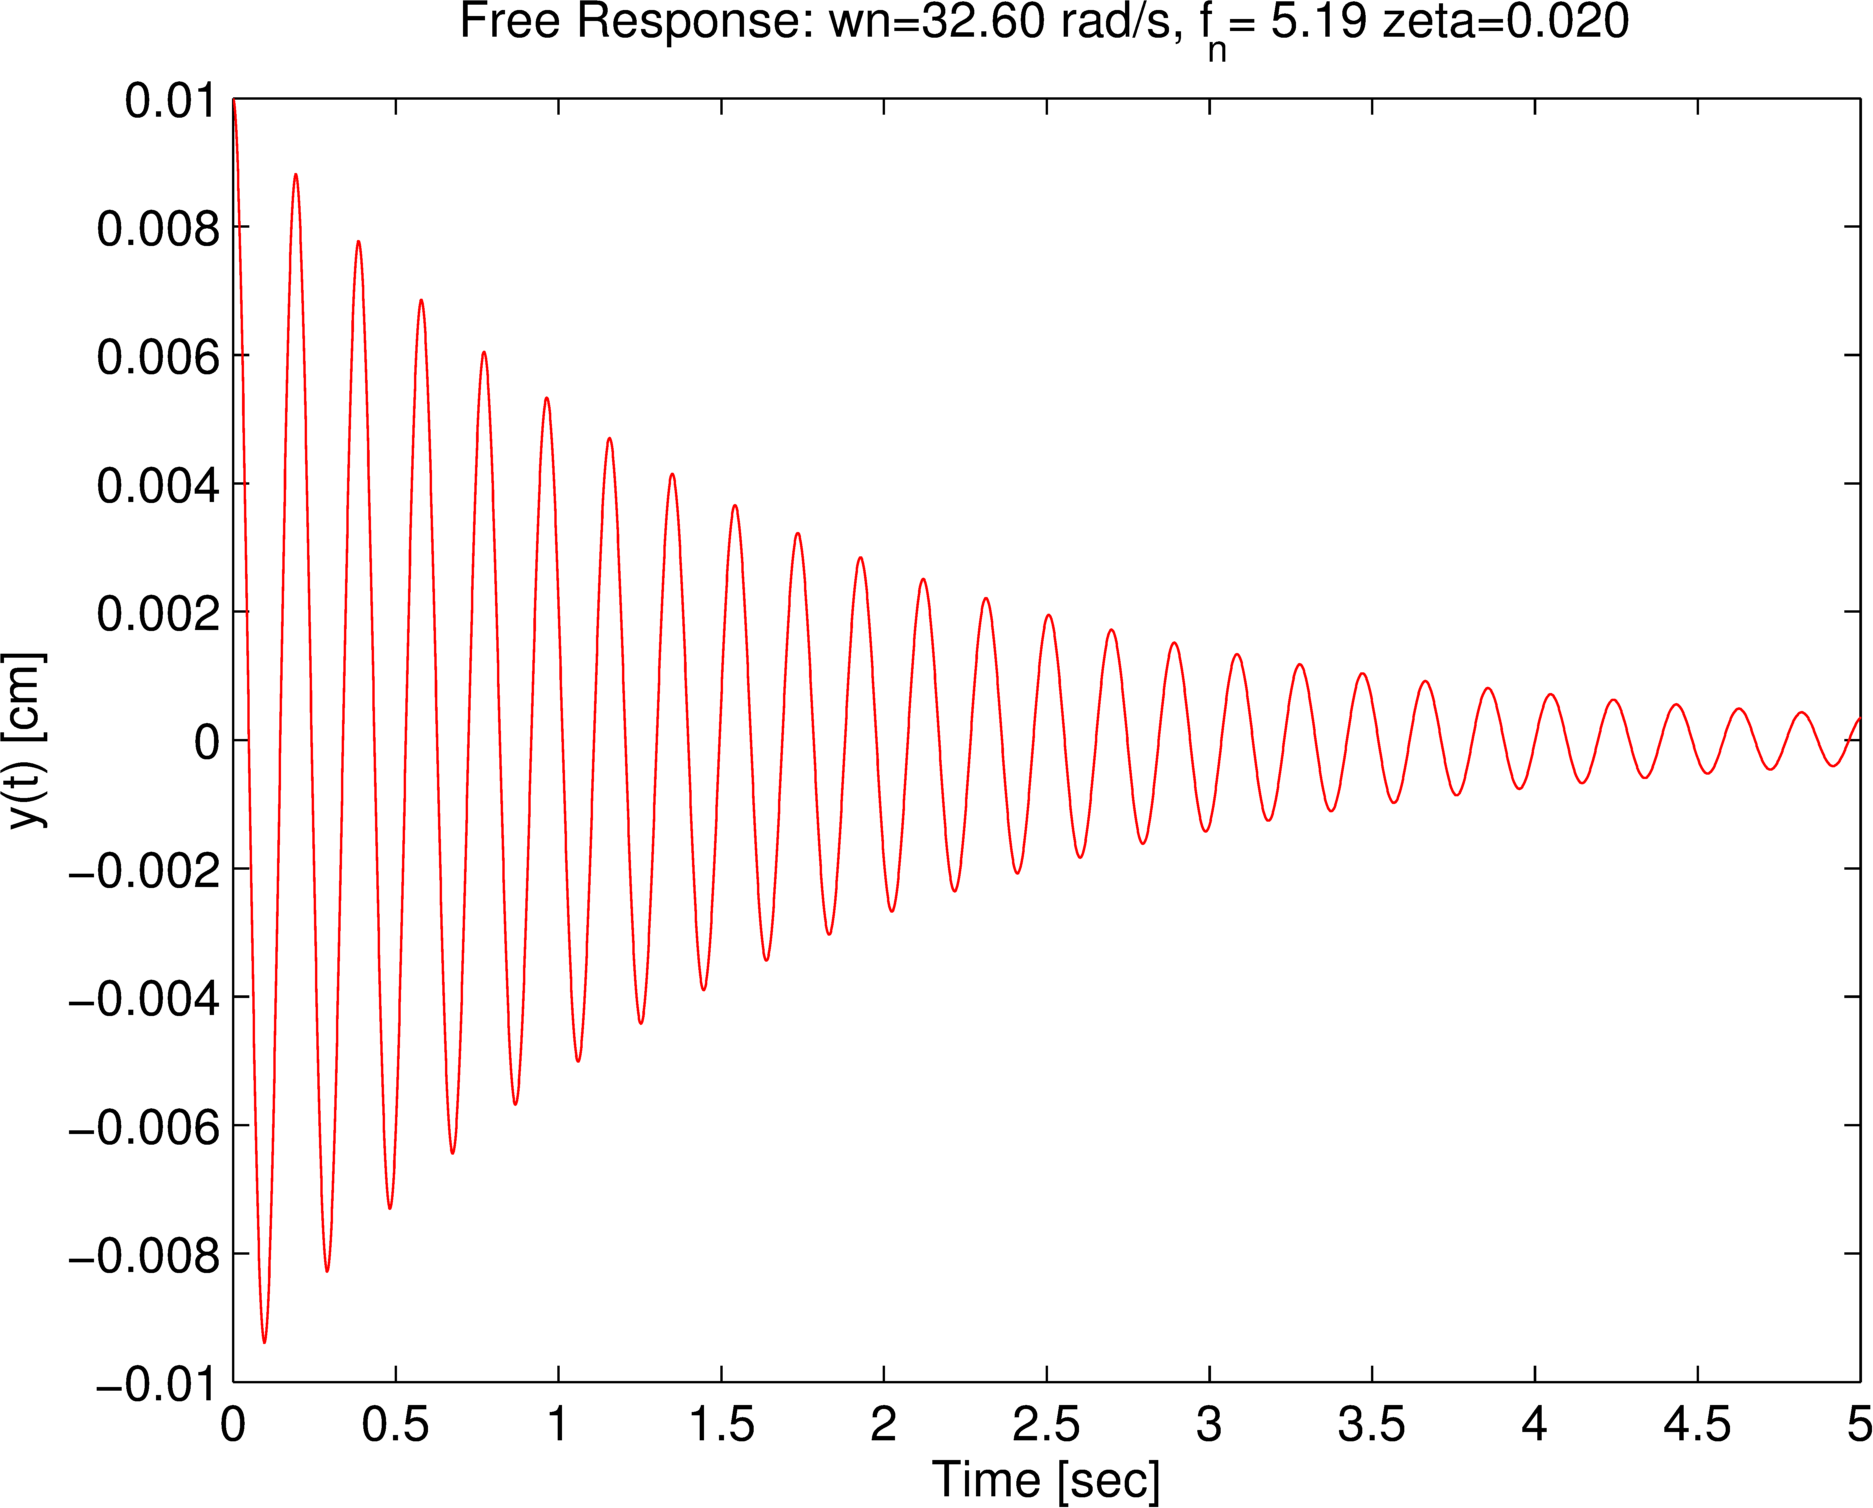
\includegraphics[width=\FigWidth\textwidth]{soln_second_free_model.png}
\caption{Graphs of the second-order free response for the predicted natural frequency from the given beam parameters.}
\label{f:soln2freemodel}
\end{figure}

\end{soln}
\fi
